\documentclass{article}
\usepackage{fullpage}
\usepackage{indentfirst}
\usepackage{amsmath}
\usepackage{amsfonts}
\usepackage{tipa}
\usepackage{tikz}
\usetikzlibrary{matrix}
\usepackage{gb4e}
\noautomath
\title{Sandhi Generalizations}
\author{Chris Oakden}
\begin{document}
\maketitle

This handout provides generalizations about a number of sandhi patterns observed in Chinese dialects as they fit into a larger typology (taken directly from Chen (2000)). The range of sandhi patterns are divided into three basic categories: spread/shift phenomena, dissimilatory processes, and cases of neutralization. Representative patterns are characterized using several representations, including syllable strings representing abstract tones, strings of morae, and autosegmental representations.
\section{Typology}
\subsection{Spread/Shift}
Chen (2000) divides spread/shift patterns into four basic types: contour, register, whole contour tone, and terminal node spread/shifts.\\
Zhenhai (Rose 1990), a Wu dialect, is said to be representative of contour spread. It is a six-tone system, where -q indicates a checked tone.
\begin{exe}
\ex
Zhenhai tones: \{MH, LH, HL, ML, Hq, Lq\}
\end{exe}
Sandhi patterns in the language are divided broadly into SW (`strong-weak') and WS (`weak-strong') types, based on the prominence of either the first or second syllable within a disyllabic domain. Focusing specifically on the SW patterns for now, the sandhi alternations are as follows (Chen 2000:64):\\
\begin{exe}
\ex
\begin{tabular}[t]{|r|c|l|l|}
\hline
&&  second $\sigma$ & \\
&& Long $\sigma$ CVN & Short $\sigma$ CVq \\
\hline
first $\sigma$ & MH & 334-51 & 334-5 \\
& LH & 115-51 & 114-5 \\
& HL & 44-31 & 44-32 \\
& ML &&\\
& Hq & 5-51 & 5-5 \\
& Lq &&\\
\hline
\end{tabular}
\end{exe}
The surface form of the rightmost syllable varies based on its syllabic structure, either long (CVN) or short (CVq). For each syllable type, there are two surface sandhi forms: \{51, 31\} and \{5, 32\}, respectively. Chen describes these alternations as "transparently a rightward migration of the tone contour from the prominent to the weak syllable which has lost its lexically associated tone" (65). In other words, the `weak' syllable de-associates from its lexically-specified tones, resulting in a default [L] tone, and the rightmost tone of the first syllable spreads to the right one mora, yielding the observed surface forms. \par
This process can be represented at a higher level of abstraction, in terms of strings of syllables. Each of the six citation tones and four sandhi forms are assigned an arbitrary symbol from an alphabet.
\begin{exe}
\ex
\label{x:zhenhaiabst}
\begin{tabular}[t]{|c|c|}
\hline
Tone & Symbol\\
\hline
MH & a\\
LH & b\\
HL & c\\
ML & d\\
Hq & e\\
Lq & f\\
51 & g\\
31 & h\\
5 & i\\
32 & j\\
\hline
\end{tabular}
\end{exe}
The well-formed strings (of length 2) in the Zhenhai SW pattern are thus:
\begin{exe}
\ex
$\mathcal{G}_{ZH}$ = \{ag, bg, ch, eg, ai, bi, cj, ei (...)\}
\end{exe}
All other possible combinations of these symbols are ill-formed. This includes any citation tone in non-initial position, sandhi forms in initial position, and unattested combinations of citation and sandhi tones:
\begin{exe}
\ex
$\mathcal{S}_{ZH}$ = \{aa, ab, ac, ad, ae, af, ah, aj, ba, bb, bc, bd, be, bf, bh, bj, ca, cb, cd, ce, cf,
cg, ci, da, db, dc, dd, de, df, dg, dh, di, dj, ea, eb, ec, ed, ee, ef, eh, ej, fa, fb, fc, fd, fe, ff, fg,
fh, fi, fj, ga, gb, gc, gd, ge, gf, gg, gh, gi, gj, ha, hb, hc, hd, he, hf, hg, hh, hi, hj, ia, ib, ic, id, ie, if, ig, ih, ii, ij, ja, jb, jc, jd, je, jf, jg, jh, ji, jj\}
\end{exe}
This method of representation captures all prohibited sequences of SW disyllables, but questions remain as to how the sandhi forms should be represented in terms of H,M,L segments and whether redundancies arise as a result.  \par
The Zhenhai data can also be represented as strings of morae which associate to tones. This representation assumes bimoracity of long syllables and monomoracity of short (checked) syllables. The ill-formed sequences in (\ref{x:szhm}) are limited to possible combinations of citation tones.
\begin{exe}
\ex
\label{x:szhm}
$\mathcal{S}_{ZH}$ = \{MHMH, MHLH, MHML, MHL, LHMH, LHLH, LHML, LHL, HLMH, HLLH, HLHL, HLL, MLMH, MLLH, MLHL, MLML, MLM, HMH, HML, HL, LMH, LLH, LHL, LML, LH\} 
\end{exe}
This characterization is problematic; two prohibited strings in this set are in fact well-formed structures. Disyllabic sequences of high and low checked tones are represented by [HL] and [LH], respectively. These strings of morae correspond to grammatical outputs (the sandhi tone for long W syllables and the citation tone for rising tone on S syllables). This representation cannot adequately distinguish grammatical and ungrammatical SW sequences in Zhenhai. \par
Chen proposes autosegmental representations of the Zhenhai data to characterize the shift of the rightmost tone on a contour to the prosodically-weak syllable in the SW constructions:

\begin{exe}
\ex
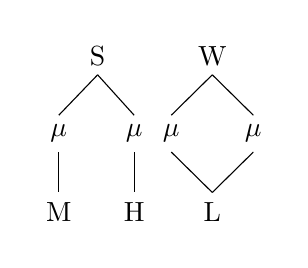
\begin{tikzpicture}[baseline=(m-1-2.base)]
\matrix (m) [matrix of nodes, row sep = 1.5em] {
	              & S &             & &           &  W  &              	   \\
	   $\mu$ &    & $\mu$ & &$\mu$&       & $\mu$                \\
	   M        &    &    H      &  &         &   L   &                            \\
};
\draw (m-1-2.south) -- (m-2-1.north);
\draw (m-1-2.south) -- (m-2-3.north);
\draw (m-2-1.south) -- (m-3-1.north);
\draw (m-2-3.south) -- (m-3-3.north);
\draw (m-1-6.south) -- (m-2-5.north);
\draw (m-1-6.south) -- (m-2-7.north);
\draw (m-2-5.south) -- (m-3-6.north);
\draw (m-2-7.south) -- (m-3-6.north);
\end{tikzpicture}
$\rightarrow$
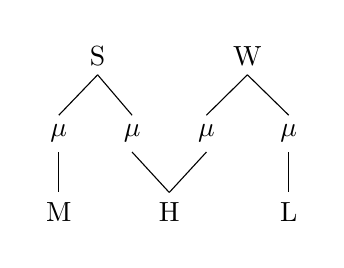
\begin{tikzpicture}[baseline=(m-1-2.base)]
\matrix (m) [matrix of nodes, row sep = 1.5em] {
	              & S &             &      &           &  W  &              	   \\
	   $\mu$ &    & $\mu$ &      &$\mu$&       & $\mu$                \\
	   M        &    &             & H  &         &        &    L                            \\
};
\draw (m-1-2.south) -- (m-2-1.north);
\draw (m-1-2.south) -- (m-2-3.north);
\draw (m-2-1.south) -- (m-3-1.north);
\draw (m-2-3.south) -- (m-3-4.north);
\draw (m-1-6.south) -- (m-2-5.north);
\draw (m-1-6.south) -- (m-2-7.north);
\draw (m-2-5.south) -- (m-3-4.north);
\draw (m-2-7.south) -- (m-3-7.north);
\end{tikzpicture}
\end{exe}
Two assumptions are apparent in this representation. Syllable nodes which head TBU morae are specified as either strong or weak in the representation. Additionally, weak syllables are assumed to contain a single L element on the melodic tier and two associations. With these assumptions, however, the autosegmental representations not only capture sandhi alternations on SW sequences, but also disambiguate grammatical and ungrammatical structures, avoiding the confounds observed when representing these processes in terms of strings of morae (\ref{x:disambiguate}):
\begin{exe}
\ex 
\label{x:disambiguate}
\begin{tikzpicture}[baseline=(m-1-2.base)]
\matrix (m) [matrix of nodes, row sep = 1.5em] {
	& $\sigma$ &      \\
	$\mu$ && $\mu$ \\
	H && L \\
};
\draw (m-1-2.south) -- (m-2-1.north);
\draw (m-1-2.south) -- (m-2-3.north);
\draw (m-2-1.south) -- (m-3-1.north);
\draw (m-2-3.south) -- (m-3-3.north);
\end{tikzpicture}
~(Grammatical)
\hspace{1cm}
\begin{tikzpicture} [baseline=(m-1-1.base)]
\matrix (m) [matrix of nodes, row sep = 1.5em] {
	$\sigma$ &\hspace{1.5em}& $\sigma$ \\
	$\mu$ & & $\mu$ \\
	H && L \\ 
};
\draw (m-1-1.south) -- (m-2-1.north);
\draw (m-2-1.south) -- (m-3-1.north);
\draw (m-1-3.south) -- (m-2-3.north);
\draw (m-2-3.south) -- (m-3-3.north);
\end{tikzpicture}
~(Ungrammatical)
\end{exe}
Important to note here is that distinguishing the two \emph{requires} specifying the root syllable node in the representation; from the moraic tier downward, the two structures are identical. \par
Wenzhou whole-tone shift (maybe)
\subsection{Dissimilation/Substitution}
Dissimilation, especially contour dissimilation, is very common in Chinese tone sandhi patterns (Chen 2000:80). A simple case of dissimilatory processes in disyllabic sandhi is observed in the Tianjin dialect of Mandarin (Li \& Liu 1995, Shi 1990).\footnote{The complexity of Tianjin sandhi processes increases substantially in trisyllabic compounds. Discussion here is simplified and limited to disyllabic forms.} The basic cases are described below, with `F' and `R' representing falling and rising contour tones.
\begin{exe}
\ex
\label{x:Tianjin1}
\begin{tabular}[t]{ccc}
 Input && Output \\
 \hline
LL & $\rightarrow$ & RL \\
RR & $\rightarrow$ & HR \\
FF & $\rightarrow$ & LF \\
FL & $\rightarrow$ & HL \\
\end{tabular}
\end{exe}
Utilizing the representation in (\ref{x:Tianjin1}) results in a straightforward characterization of ungrammatical sequences of disyllables.
\begin{exe}
\ex
\label{x:TJsyl}
$\mathcal{S}_{TJ}$ = \{LL, RR, FF, FL\}
\end{exe} 
As strings of morae with associating to H and L tones only, prohibited structures can also be represented without any confounds.
\begin{exe}
\ex
\label{x:TJmor}
$\mathcal{S}_{TJ}$ = \{LLLL, LHLH, HLHL, HLLL\}
\end{exe} 
Curiously, though, representation of segments on the melodic tier (again using only H and L) fails to isolate ungrammatical sequences.
\begin{exe}
\ex
$\mathcal{S}_{TJ}$ = \{LL, LHLH, HLHL, HLL\}
\end{exe}
A sequence of falling + rising tones (HLLH) is predicted to be ungrammatical in the melodic representation; two of its substrings (LL and HLL) are in the set of prohibited strings of melodic elements. It appears that some reference to the syllable as a unit is necessary, either as a 1-to-1 syllable and symbol correspondence as in (\ref{x:TJsyl}), or by representing level tones (on the syllabic level) as associations to two morae (\ref{x:TJmor}). Full autosegmental representations also succeed in making this distinction, even without reference to a syllable root node.
\begin{exe}
\ex
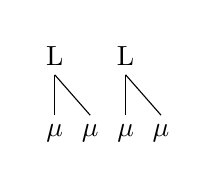
\begin{tikzpicture}[baseline=(m-1-1.base)]
\matrix (m) [matrix of nodes, row sep = 1.5em)] {
L & & L & \\
$\mu$ &$\mu$ & $\mu$ & $\mu$ \\
};
\draw (m-1-1.south) -- (m-2-1.north);
\draw (m-1-1.south) -- (m-2-2.north);
\draw (m-1-3.south) -- (m-2-3.north);
\draw (m-1-3.south) -- (m-2-4.north);
\end{tikzpicture}
~(Ungrammatical)
\hspace{1cm}
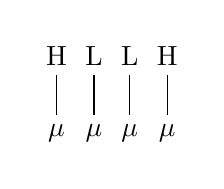
\begin{tikzpicture}[baseline=(m-1-1.base)]
\matrix(m)[matrix of nodes, row sep = 1.5em] {
H & L & L & H \\
$\mu$ & $\mu$ & $\mu$ & $\mu$ \\
};
\draw (m-1-1.south) -- (m-2-1.north);
\draw (m-1-2.south) -- (m-2-2.north);
\draw (m-1-3.south) -- (m-2-3.north);
\draw (m-1-4.south) -- (m-2-4.north);
\end{tikzpicture}
~(Grammatical)
\end{exe}
Also the Nanjing dialect case?
\subsection{Neutralization/Differentiation}
Neutralization of lexical tone contrasts is pervasive in Chinese dialects. This is especially common in Wu dialects, where only the citation tone of the first syllable in a domain is retained, and tones on all other syllables are neutralized. An example of neutralization in a disyllabic context comes from Zhangping, a southern Min dialect spoken in Fujian (Zhang 1982), with seven lexical citation tones, and three sandhi tones, given in Chao tone number form.
\begin{exe}
\ex
Zhangping tones: \{24, 11, 5q, 53, 53q, 31, 21 (citation tones), 33, 55, 21 (sandhi tones)\}
\end{exe}
Disyllabic tone sandhi is as below; initial tones in a disyllabic domain neutralize to one of three sandhi forms, while final tones do not alter.
\begin{exe}
\ex
\begin{tabular}[t]{c|r|c|c}
&& second $\sigma$ & \\
\hline
&& 24, 11, 5q, 53, 53q & 31, 21 \\
\hline
first $\sigma$ & 24 & & \\
& 11 && \\
& 21 & 33-T & 55-T \\
& 5q && \\
\hline
& 31 && \\
& 53 & 21-T & \\
& 53q && \\
\end{tabular}
\end{exe}
As abstract syllable-level tones, representation with arbitrary symbols (as in (\ref{x:zhenhaiabst})) is straight forward. Any combination of two citation tones is ill-formed, as are any with sandhi tones in final position. Such a representation would adequately select ungrammatical sequences of two tones. \par
In terms of H,L, and M segments, however, representation is problematic. The tones with the phonetic forms [31, 21, 11] evade a clear phonological characterization in this framework:
\begin{exe}
\ex
\begin{tabular}[t]{cc}
Phonetic Form & Phonological Form  \\
\hline
31 & ML  \\
\textbf{21} & \textbf{ML?  LL?} \\
11 & LL \\
\end{tabular}
\end{exe}
Assigning [ML] and [LL] to [31] and [21] respectively is a reasonable assumption given the phonetic forms. However, this leaves no option for [21], which is claimed to be a separate lexical tone from the others. One possibility is [MM], a less reasonable option by comparison, but this creates a confound with the sandhi tone [33] for which [MM] appears to be the best fit. \par
Without distinct phonological representations of these tones, it is not possible to represent the observed sandhi patterns in terms of sequences of tones on the melodic tier, strings of morae, or even autosegmental representations. Neither Chen (2000) nor Zhang (1982) offer a phonological representation for these tones.
\section{Next Steps}
\begin{itemize}
	\item Representing domain-wide spread in Shanghai and other Wu dialects
	\item Approaches in OT
	\item Case studies: Changting, New Chongming, Wuxi, Danyang, Nantong, Xiamen (do I need this?), Wenzhou
\end{itemize}
\newpage
\begin{center}
References
\end{center}
Chen, Matthew. 2000. \textit{Tone Sandhi: Patterns across Chinese Dialects}. Cambridge: CUP. \\
Li, Xinjian \& Liu Sixun. 1985. Tianjin fangyan de liandu biandiao. \textit{Zhongguo Yuwen} 1. 76-80. \\
Shi, Feng. 1990. Hanyu he Dong-Tai yu de Shengdiao Geju. PhD Dissertation, Nankai University. \\
Zhang, Zhenxing. 1982. Zhangping (Yongfu) de liandu biandiao. \textit{Fangyan} 1982. 175-196.\footnote{I looked back and checked this source, and it's not even there. There is an article about this dialect in that particular issue, but it's just a basic description of initials/finals/tones as well as a long list of homophones. I did not find any discussion of sandhi in the paper.}

\end{document}